\Chapter{Koncepció}

A legtöbb társasjátékban a jól ismert hat oldalú dobókockát használjuk véletlen számok generálására.
Az első híresebb kivétel a \textit{Dungeons and Dragons}\cite{dnd} nevű szerepjáték volt, ahol minden szabályos testből képzett dobótesteket használtak véletlen számok generálására.
A platóni testek mellett használnak két tíz oldalú trapezoédert, amelyek segítségével tudnak nulla és kilencvenkilenc között egyenletes eloszlással választani véletlen számokat.
Ezeket a kockákat szinte csak szerepjátékokban használják, és gyakran több kocka dobásának az összegét veszik kapott értéknek.

\begin{figure}[h!]
	\centering
	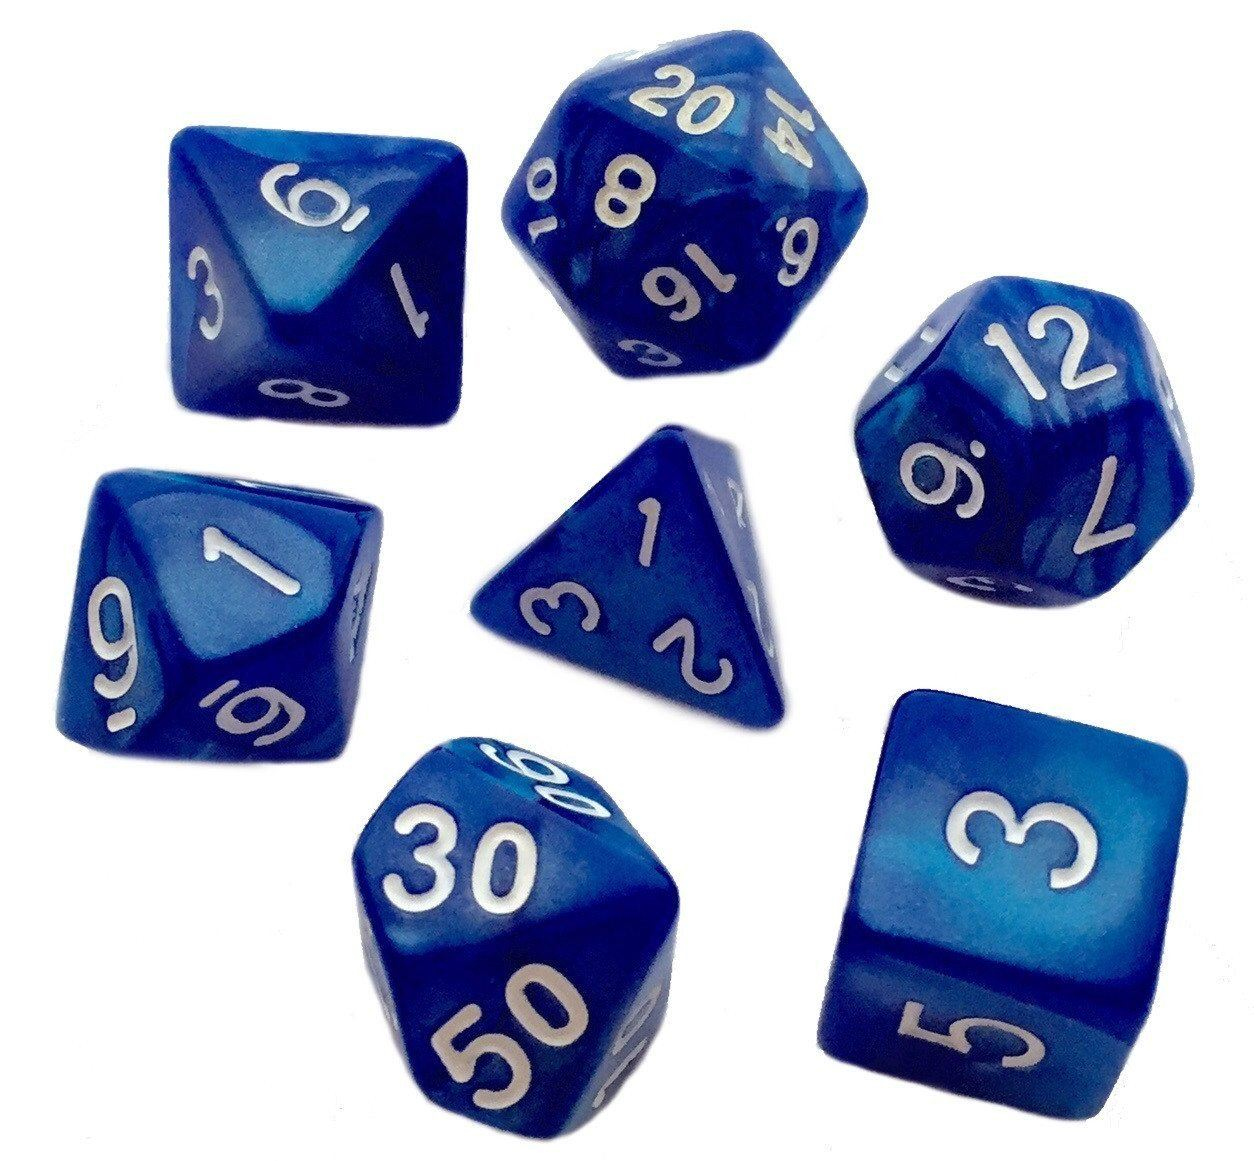
\includegraphics[scale=0.15]{images/diceset.png}
	\caption{A legtöbb szerepjátékban használt dobókockák.}
	\label{fig:diceset}
\end{figure}

Ezzel szemben az újonnan kiadott társasjátékok csak a hagyományos kocka alapú dobótesteket használják.
Ez a fajta korlátozás gyakran unalmas játékmenetet eredményez, vagy túl sok minden fog múlni egyetlen dobáson.
Ennek a kiküszöbölését három különböző módon lehet megtenni:
\begin{enumerate}
\item A szabályok egyengetése, egyensúlyozása, hogy ne legyen érezhetően nagy szerepe a véletlen számoknak.
\item A dobókockán szereplő szimbólumok módosításával változtatnak az eloszláson.
\item Egyedi alakú dobótestek használata.
\end{enumerate}

A legtöbb játékban igyekeznek az 1. pontot követni, ami gyakran nem a legjobban sikerül.
De ez nem lehetetlen, mert például az \textit{Axis and Allies}\cite{axisnallies} második világháborús stratégiai játék ezt sikeresen tudta elérni.
A katonai egységek különböző költségeivel, harci statisztikáikkal valamint az egyedi harcrendszerével egy könnyen megtanulható, nehezen $mesterelheto$ de mégis megunhatatlan játékélményt elérni.
Ezek miatt több múlik a játékosok stratégiáján, mint a tényleges kockadobásokon.

A 2. pontban említett módszert gyakran csak arra használják, hogy egyedi oldalak legyenek a kockákon, és a tényleges eloszlást nem változtatják meg.
A \textit{Dark Souls: The Board Game}-ben \cite{darksouls} használt dobókockák viszont kifejezetten jó példák az oldallapokon lévő szimbólumok lecserélésére.
A sebzések számításához használt három különböző színű kocka (fekete, kék és narancssárga) várható értékei egy konstans értékkel nőnek, valamint a dobható értékek tartománya is nő ezzel együtt.
A szabályrendszernek hála a játék ugyan azt az élményt adja, mint a videojáték testvére.
Többet számítanak a játék során a megszerzett tárgyak, játéktapasztalat mint a játékosok szerencséje.

\begin{figure}[h!]
	\centering
	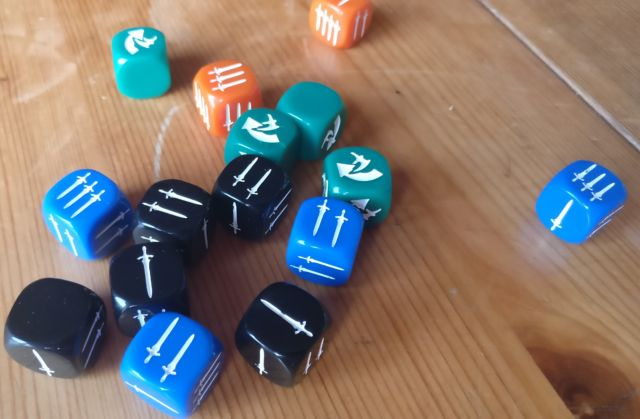
\includegraphics[scale=0.6]{images/dsdice.png}
	\caption{A \textit{Dark Souls: The Board Game}-ben használt dobókockák.}
	\label{fig:dsdice}
\end{figure}

A harmadik megoldást egyetlen társasjáték sem használja, ezért mi magunk fogunk ilyen testeket generálni, feltételezve hogy az egyes elvárt alakzatok léteznek.
A testek közelítéséhez Monte-Carlo-módszert fogunk használni, azaz egy szimulált fizikai környezetben végzünk a testekkel dobássorozatokat.
A kapott eredmények alapján fogjuk a testet módosítani, hogy az elvárt valószínűségekhez közelítsen a mért adat.